\newpage
\end{multicols}
\chapter{Quick Start Guide}
	
Welcome to the quick start quide.  Following these steps, you will get your 
gain/phase analyser up and running in no time!

\begin{figure}[h]
\centering
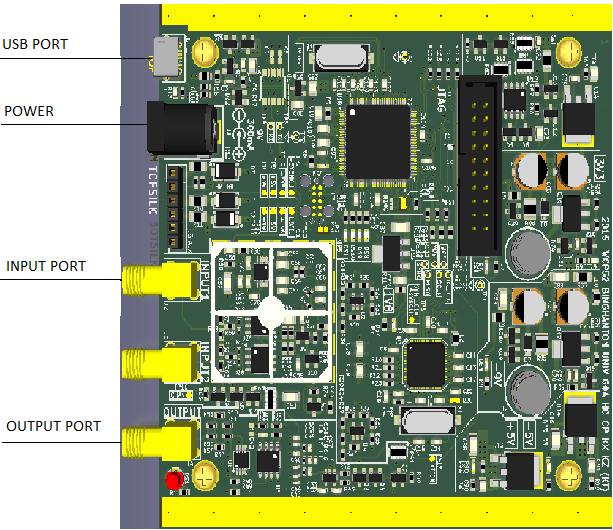
\includegraphics[width=5.5in]{getting_started/ports}
\caption{High level overview of gain/phase analyser}
\label{fig:highlevel}
\end{figure}

\section{Getting to know the device}

For the most basic use of the gain/phase analyser, you will be using the four ports described in the figure.
The USB Port is so that the device may connect to the computer.
Power is the port that you will plug the power supply into.  The board does not receive enough power from USB, so this is necessary for operation.
Input port receives signals from the filter that you are analysing.
Output port sends signals to the filter.


\section{Setting up your device}

First begin by connecting a filter to the board.  Connections for the filter must be made between the Output Port and Input Port.

Now, we will connect the device to a PC using a micro USB cable.  Place one side of the cable into the USB port and the other side into any USB port on your PC.

Now, we will provide power to the device.  Plug the power supply into the Power port.

\section{Collecting some data}

Excellent job.  Now we move to the computer where we can take a measurement and get some results!  
Go ahead and run the gain/phase analyser application.   

\begin{center}
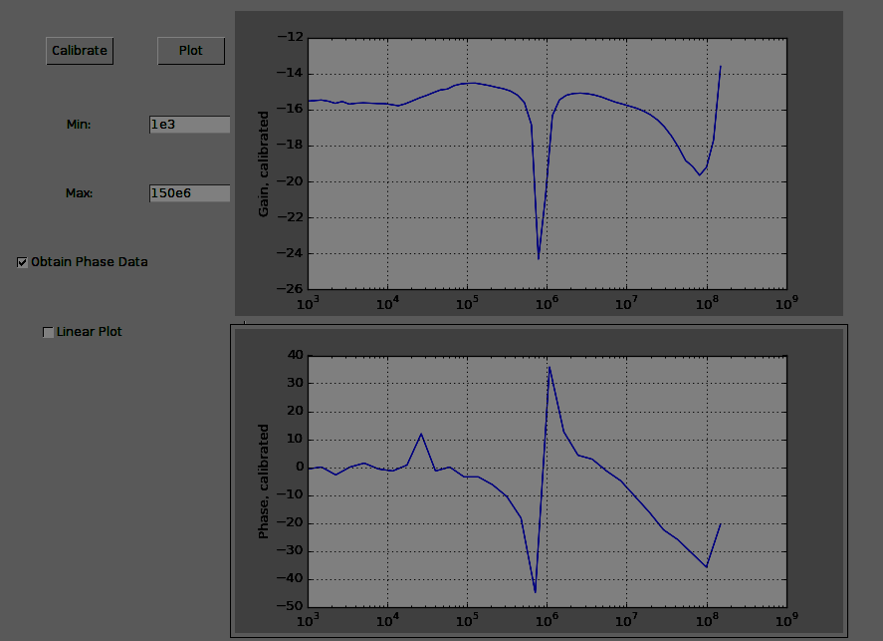
\includegraphics[width=4in]{getting_started/gui}
\end{center}

Before actually executing analysis, it is important to set the minimum and maximum frequencies to test.  These numbers are always
written in Hz.  Additionally, they may be written as a decimal number, for example, 1000 or as an exponent like 1e3.

Here, we will test from 1000 Hz up to 150 MHz, so we input 1e3 as min and 150e6 as max.  As stated earlier, we could have set min to 1000 and max to 150000000,
or any combination of these inputs.

Now we have a choice, we may calibrate the data or make our plot.  Since we are just starting out, just generate your plot and watch some pretty results pop onto your screen.  Congratualations!  You've just gotten your first plot out of our USB Gain/Phase Analyser.

\section{Calibration}

With the basics out of the way, we can talk about calibration.  We highly recommend doing this as it will provide significantly more accurate data.  It will reduce some of the noise that you will get from your set up and surrounding environment.  Note that this must be done before taking a reading with a filter connected.

In order to calibrate, you will first need to connect a wire between the output and input.  There will not be a filter in between the ports when you do the calibration.  Enter the min and max frequencies that you want to test your filter for.  If you enter different frequencies than you do when you connect your filter then your analysis will not work!  Now, simply press the calibrate button and wait for calibration to finish.

Good work on calibrating your set up.  Now connect a filter and perform the analysis as you did before.  





\begin{multicols}{2}
